% set 0.5 inch indentation
\setlength{\parindent}{0.5in} 
% set paragraph space = 0 space
\setlength{\parskip}{0mm}
% set line space 1.5
\setlength{\baselineskip}{1.6em}

\chapter{LITERATURE REVIEW}
\label{ch:literature-review}

\textit{This chapter begins with a review of the functional architecture of autonomous driving systems, coordinate systems, the PixHawk, and ROS coordinate conventions.} 

\section{Software Architecture of Autonomous Driving Vehicles}
\label{section-name-in-literature-review}

\shortciteA{sbehere16t} splits the major components of the motion control part of autonomous driving systems into three main categories as shown in Figure~\ref{fig:fav_automonous}. These categories are:

\begin{itemize}
	\item Perception of the external environment in which the vehicle operates
	\item Decision making and control of vehicle motion with respect to the external environment that is perceived
	\item Vehicle platform manipulation, which deals mostly with sensing, control, and actuation of the vehicle, with the intention of achieving the desired motion.
\end {itemize}

Each category can be further broken down into several components. I describe each component in more details in the following sections.

\subsection{Perception}

Sensing components sense the state of the vehicle and the state of the environment in which the vehicle operates. The sensor fusion component considers multiple sources of information to construct a hypothesis or belief about the state of the environment. The localization component determines the location of the vehicle with respect to a global map. The semantic understanding component processes the sensor input and derives meaningful information from it. The world model component holds the current estimate of the state of the external environment.

\subsection{Decision and Control}
The trajectory generation component repeatedly generates a set of obstacle-free trajectories in the world coordinate system and picks an optimal trajectory from the set. Energy management components deal with energy management of the vehicle. Diagnosis and fault management monitors the state of the overall system and its components. Reactive control components are used for immediate responses to unanticipated stimuli from the environment. The vehicle platform abstraction component refers to a minimal model of the vehicle platform. 

\subsection{Vehicle Platform Manipulation}

The platform stabilization component's task is to keep the vehicle platform in a controllable state during operation. Trajectory execution components are responsible for executing the trajectory generated by the decision and control component. 

\begin{figure}
	\centering
	\caption[FAV of Antonomous Driving System.]{\small 
		Functional architecture of an autonomous driving system. Reprinted from Behere (2016). }
	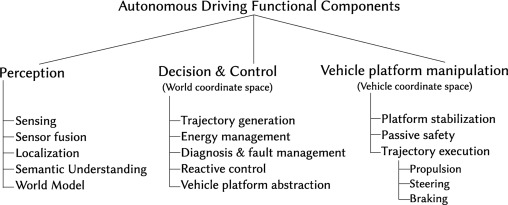
\includegraphics[width=5in]{figures/literature/fav_autonomous_driving}
    \label{fig:fav_automonous}
\end{figure}

\section{Coordinate Systems}

In this section I describe the different coordinate system conventions in use in robotic applications. 
	
\subsection{Earth Centric, Earth Fixed}

The earth-centered earth-fixed (ECEF) coordinate system, rotates with the Earth and has its origin at the center of the Earth. Refer to Figure~\ref{fig:coordinatesystem} (a) for a visualization. ECEF follows the right-handed coordinate system convention. \shortciteA{coordinatesystem} describes ECEF as follows.

\begin{itemize}
	\item The origin is at the center of mass of the Earth, a point close to the Earth's center.
	\item The Z axis is on the line between the magnetic north and south poles, with positive values increasing northward (but not exactly coinciding with the Earth's rotational axis).
	\item The X and Y axes lie in the plane of the equator.
	\item The X axis passes through the point on the equator from 180 degrees longitude (negative) to the prime meridian (0 degrees longitude, positive).
	\item The Y axis passes through the point at 90 degrees west longitude along the equator (negative) to 90 degrees east along the equator (positive).
\end{itemize}

\subsection{World Geodetic System}
The World Geodetic System is a standard system used in GPS, cartography and geodesy. The latest revision is WGS 1984 (WGS 84) that was established and is maintained by the United States National Geospatial-Intelligence Agency. It was last revised in 2004. The World Geodetic System 1984 (WGS 84) is one of the best global geodetic reference system for the Earth available presently. The datum (ellipsoid) defined by WGS 84 is generally used to convert the GPS latitudes and longitude to the UTM coordinate system.

\subsection{Universal Transverse Mercator Geopraphic Coordinate System}
The Universal Transverse Mercator (UTM) is a coordinate system that divided the earth into 60 zones. Each zone is a plane with its own x and y coordinates in meters. It ignores altitude and treats the earth as a perfect ellipsoid. A UTM coordinate has:

\begin{itemize}
        \item A zone number.
        \item A hemisphere (N/S).
        \item An easting (X coordinate).
        \item A northing (Y coordinate)
\end{itemize}

A coordinate 14.08057584 \degree N, 100.61284553 \degree E in latitude and longitude is represented as 47 N 674132 1557234 in UTM.

\subsection{Local tangent plane}

In the local tangent plane coordinate system, a position on the earth is fixed about the origin. There are two conventions as shown in Figure~\ref{fig:coordinatesystem} (b).

\begin{itemize}
	\item X=East, Y=North, Z=Up (ENU).
	\item X=North, Y=East, Z=Down (NED), which is commonly used in aviation, as the objects of interest usually lie before an aircraft (down or positive Z).
\end{itemize}

\begin{figure}%
	\centering
	\caption[ECEF coordinate system]{\small Coordinate systems. (a) Earth centric, earth fixed (ECEF) coordinate system. (b) Local tangent plane coordinate systems. Reprinted from Krishnavedala. 
	}%
	\subfloat []{{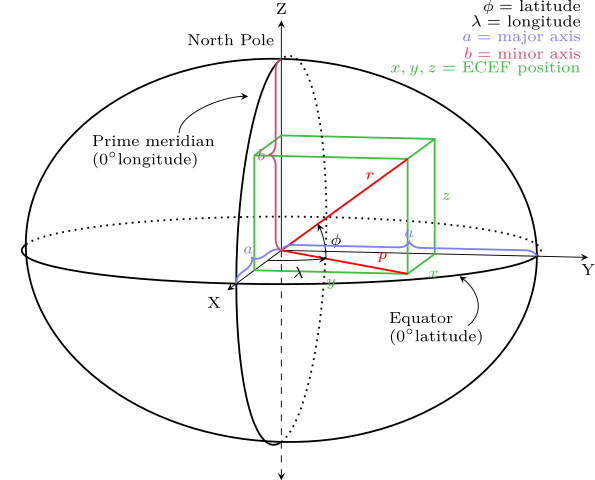
\includegraphics[width=3in]{figures/literature/ECEF}}}%
	\subfloat []{{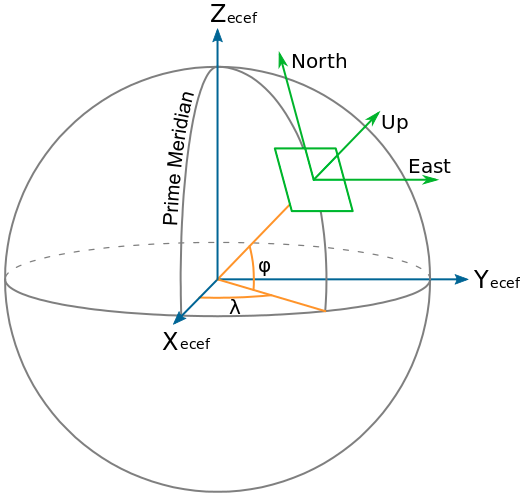
\includegraphics[width=3in]{figures/literature/ENU_NED}}}%
	\label{fig:coordinatesystem}%
\end{figure}

\subsection{PixHawk and ROS coordinate systems}

PixHawk follows the NED convention, whereas ROS follows the ENU convention. The conversion between these different conventions is handled automatically by MAVROS. To translate air-frame related data, a rotation of $180^{\circ}$ degrees is applied about the roll (X) axis. For local data, a $180^{\circ}$ rotation is applied about the roll (X) and $90^{\circ}$ rotation is applied about the yaw (Z) axes.

It is good practice in ROS to set up reference frames as described by \shortciteA{rosrefframes}, shown in Figure~\ref{fig:rosrefframes}.

\begin{itemize}
	\item The coordinate frame called base\_link is rigidly attached to the mobile robot base. It can be attached in any arbitrary position or orientation.
	\item The coordinate frame called odom is a world-fixed frame. The pose of a robot is continuous in this frame, but it can drift over time.
	\item The coordinate frame called map is a world fixed frame, with Z-axis pointing upwards. 
	\item The coordinate frame called earth is the origin of the ECEF frame.
\end{itemize}

\begin{figure}
	\centering
	\caption[Relation between ROS frames]{\small 
		Relationship between ROS frames. Reprinted from \shortciteA{rosrefframes}. }
	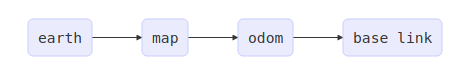
\includegraphics[width=5in]{figures/literature/ros_rel_frames}
	\label{fig:rosrefframes}
\end{figure}

\section{Wireless Mesh Network}

A wireless mesh network's (WMN) consists of two types of nodes, mesh routers and mesh clients. Mesh routers form the mesh backbone for mesh clients. Every node in the mesh has the capability to route packets forward for other nodes if the packet destination is not in direct wireless transmission range. Mesh routers provide functionality as bridge/gateway that enables the WMN to integrate with other networks such as cellular, ad-hoc and ethernet. In a wireless mesh network, all the participating nodes automatically establish and maintain mesh connectivity and are in effect dynamically self-organized and self-configured. WMN can be rapidly deployed where there is no network coverage and has the potential for application in disaster management.

\subsection{WMN Network Architecture}

A wireless mesh network has two types of nodes, mesh routers and mesh clients. Mesh routers can have multiple networking interfaces to provide bridge/gateway functionality to the mesh network and have additional routing functions to support mesh networking. Mesh routers can be built on similar hardware platform as a conventional wireless router. Mesh routers can be build based upon embedded systems and general-purpose computer systems. Mesh clients have capability for mesh networking and can also work as a mesh router, nevertheless they lack bridge/gateway function and usually have only one wireless interface.


The architecture of WMNs can be classified into three types based upon the composition of mesh routers and clients.

\begin{itemize}
	\item \textit{Infrastructure/Backbone WMNs.}
	In this architecture mesh routers form an infrastructure for clients that connect to them. The mesh routers automatically establish and maintain links between themselves and provide gateway functionality to connect the mesh network to other networks and the internet. 
	
	\item \textit{Client WMNs.} In this architecture, mesh routers are not required for maintaining a mesh network. Mesh clients provide peer-to-peer networking, performing routing and configuration management. A packet may reach the destination node through multiples hops through client nodes.
	  
	\item \textit{Hybrid WMNs.} In this architecture, mesh routers provide infrastructure backbone with access to other networks. Client nodes can connect to the mesh network through meshing with other clients, as well as through mesh routers. This in effect, is a combination of infrastructure and client WMNs, and provides increased connectivity and coverage.
\end{itemize}

\subsection{Features of WMNs}

WMNs have redundant nodes and can provide high level of fault tolerance and robustness. If the case of link failure, the mesh network can adapt and reroute the data. Using multi-hop strategies, the coverage range can be increased, as intermediate router and clients can relay packets between hosts which do not have a direct line of sight. WMNs can be rapidly deployed with less maintenance because of self-forming, self-healing and self-organization capability. They are compatible with ad-hoc wireless clients.


\subsection{Routing Protocols for WMNs}

WMNs has redundant and mobile clients, hence, the routing protocols should find and maintain routes between the source and destination nodes by detecting and responding to changes in network topology. Ideally routing protocols should maximize the capacity of the network and minimize the packet delivery delays by creating and selecting efficient routes between nodes.

Wireless mesh routing protocols can be classified into three categories:

\begin{itemize}
	\item \textit{Proactive Routing Protocol.} Proactive routing protocols build and maintain the routing table by sharing routing data among nodes at periodic intervals. It selects the route from the routing table while forwarding packets from one node to the other. Optimized Link State Routing Protocol (OLSR) and Better Approach to Mobile Ad-hoc Networks (BATMAN) falls under this category.
	\item \textit{Reactive Routing Protocol.}  Reactive routing protocols searches the route from source to destination node on demand as it is required. Examples of this category are Ad Hoc On-Demand Distance Vector Protocol (AODV) and Dynamic Source Routing Protocol (DSR).
	\item \textit{Hybrid Routing Protocol.} Hybrid Routing Protocol uses both reactive and proactive routing strategies depending upon the environment. As a reactive routing protocol, it will provide the path on demand, based on up-to-date information. Examples of hybrid routing protocols are ZRP (zone routing protocol), HSLS (hazy sighted link state routing protocol).
\end{itemize}

\subsubsection{Comparision of Routing Protocols}

\shortciteA{Mbarushimana2007} does a comparative study between the performance of reactive (AODV and DSR) and proactive (OSLR) protocols. They run simulations for 1000 seconds, considering four different scenerios, namely, workload, number of flows, number of nodes in the network, and node movement speed. The performance of the three routing protocols is measured based on throughput, good-put, routing load and end-to-end delay. They come to the conclusion that OSLR shows the best performance in terms of data delivery ratio and end-to-end delay, and provide insight that network layer tends to drop more packets while reactive protocol is computing the route to the destination. In their study OSLR still outperforms the reactive routing protocols at higher speeds even though it has the highest routing overhead due to its exchange of periodic routing updates.

\shortciteA{Kulla2012} does a performance comparison of OSLR and BATMAN routing protocols in an indoor stairs environment of 5 floor building. They come to the conclusion that both the protocols perform well for one-hop and two-hop communication. The delay and packet loss increased after three hops for static node scenario and after two hops for moving node scenario. BATMAN performs better than OSLR for packet loss metrics because BATMAN buffers packets when routes are unstable. In general, OSLR protocol showed better performance than BATMAN protocol. OSLR shows better performance than BATMAN regarding the delay metrics, which is critical for real-time communication between a cluster of drones.

From these studies of performance comparisons OSLR seems to be the most suited to my use case, as:
\begin{itemize}
	\item Proactive protocols (OSLR) performs better than reactive protocols in terms of data delivery ratio and end-to-end delay.
	\item Reactive protocols tends to drop packets while they are computing the route.
	\item OSLR shows better performance than BATMAN for delay metrics.
	\item Latest information about the drones in the mesh network is more critical than stale information, which means OSLR with less delay is more suited to the use case of my study.
\end{itemize}

\subsection{Optimized Link State Routing Protocol}

Optimized Link State Routing Protocol (OSLR) belongs to the class of link state routing protocol, with optimization for mobile ad hoc networks.  It is a distributed protocol with no central agency that exchanges topology information with other node of the network periodically. Each node maintains a routing table, and is a proactive protocol. When data is to be sent, it refers to the routing table. The route to other nodes are maintained by each node proactively. 

HELLO message is used for link sensing, neighbor detection, and multipoint relay (MPR) selection. HELLO messages are not forwarded by the nodes. The nodes in OSLR use only selected nodes called multipoint relay (MPR) to re-transmit control messages, reducing overhead from control messages flooding the network. Each node in the network selects a set of nodes in its symmetric 1-hop neighborhood called MPR set of that node. Neighbors which do not belong to MPR set of the node receive and process broadcast messages but do not re-transmit it. If an interface of a node has at least one verified bi-directional link with an interface of another node, it is considered as its symmetric 1-hop neighbor. 

Topology Control (TC) message is used to disseminated topology information through the network, using optimized flooding through MPR mechanism. The TC messages distributed to each node is used to calculate routing table in each node.

If a node has multiple interfaces, it must announce, periodically, information describing its interface configuration to other nodes in the network. Multiple Interface Declaration (MID) message is flooded by such nodes using MPR mechanism in the network, and is used for routing table calculations.

Gateway/bridge nodes have non OSLR interfaces connected to external network such as the ethernet. Host and Network Association (HNA) message are periodically broadcasted by such nodes to register such routing information in the routing table.


The role of OSLR is not to forward data packets. It maintains the routing table in each node which is used by the system to perform network layer forwarding function.

\subsection{FANET}

Flying ad hoc network (FANET) is a specialized subset of mobile ad hoc network(MANET). FANET takes into consideration the challenges faced by MANET with flying UAVs as the mesh nodes. FANET can also be classified as a subset of Vehicular ad hoc network (VANET), where the mesh nodes are vehicles on the ground. The relation between MANET, VANET and FANET is given in Figure~\ref{fig:manet-vanet-and-fanet}.

\begin{figure}
	\centering
	\caption[MANET, VANET and FANET]{\small 
		MANET, VANET,and FANET Reprinted from \shortciteA{Tareque2015}. }
	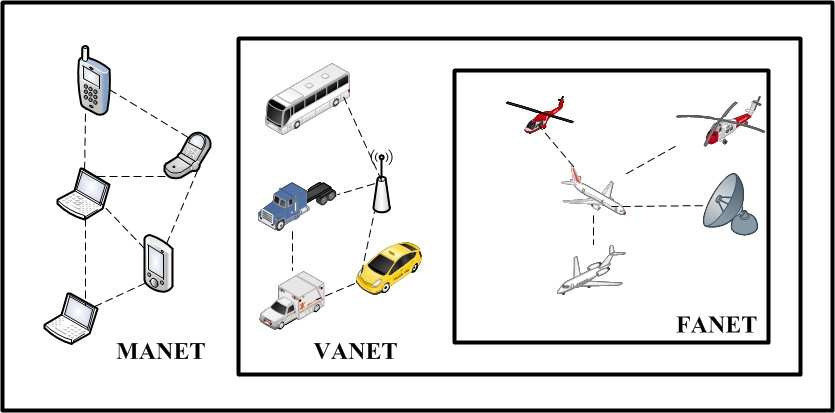
\includegraphics[width=5in]{figures/literature/MANET-VANET-and-FANET}
	\label{fig:manet-vanet-and-fanet}
\end{figure}

Surveys of FANET has been carried out by \shortciteA{Chriki2019} and \shortciteA{Tareque2015}. The challenges of FANET described can be summarized as follows:

\begin{itemize}
	\item \textit{Network topology change.} In FANET, rapidly moving UAVs changes the network topology more frequently.
	\item \textit{Node mobility.} UAVs have a higher degree of mobility than vehicles or people on ground. Node mobility issues can be considered as the most significant difference between FANET and other ad hoc networks.
	\item \textit{Node density.} Node density in FANET is lower than other MANETs. FANET nodes are spread across the sky. There are less number of average nodes in a unit area in FANET. 
	\item \textit{Radio propagation model.} MANET and VANET nodes are close to the ground and because of the environment, they may not have direct line of sight. FANET nodes are in the sky and for most cases have direct line of sight between the nodes.
	\item \textit{Power Consumption.} For large UAVs power consumption is not a significant factor when designing the FANET. However for small UAVs the power consumed by FANET must be taken into consideration.  
	\item \textit{Localization.} UAVs because of its higher mobility degree may have inaccurate GPS position information as compared to other MANETs.	
\end{itemize}

Routing protocols for FANET follows similar classification as WMNs and are as follows:

\begin{itemize} 
	\item \textit{Static protocols.} These protocols have fixed routing tables.
	\item \textit{Proactive protocols.} Updates the routing tables periodically.
	\item \textit{Reactive protocols.} Finds path to the destination node when data needs to be sent.
	\item \textit{Hybrid protocols.}  These use both reactive and proactive strategies when required. 
	\item \textit{Geographic based protocols.} These protocols use position information.
\end{itemize}

There are multiple optimization and extensions for OSLR specifically done to solve challenges for FANET. Some of them are:

\begin{itemize}
	\item \textit{DOLSR.} \shortciteA{Alshabtat2011} proposes Directional Optimized Link State Routing Protocol (DOLSR) which uses directional antenna and heuristic to minimize the number of MPRs. They show reduced end-to-end delay and enhanced overall throughout using DOLSR for FANET.
	\item \textit{P-OSLR.} \shortciteA{Rosati2013} proposes Predictive OSLR (P-OSLR) that uses GPS information to help the routing protocol. It take the relative speed between the nodes in account to calculated expected transmission count (ETX) metric. This metric is used by OSLR for link quality sensing. The show increased multi-hop reliability with minimum outage time as compared to OSLR in FANET environment.
	\item \textit{ML-OSLR.} \shortciteA{Zheng2014} proposes Mobility and Load aware OSLR (ML-OSLR) that introduces mobility and load aware algorithm in the routing protocol. ML-OLSR does not select high speed nodes as the MPR and avoid routing through high load, congested and high speed nodes to increase network stability. They show increased performance in packet delivery ratio and average end-to-end delay compared to OSLR with FANET based simulation.
\end{itemize}

\shortciteA{Singh2015} presents the application of OSLR to FANET under different mobility model of the nodes through simulation. He shows that the increase in speed of nodes decreases throughout, increases end-to-end delay and decreases packet delivery ratio for most mobility model. However, for my study, the speed of the node are relatively low, and nodes spend most of their time waiting for other nodes to arrive to their way-point and take picture, therefore I shall purse the use of generic OSLR for this thesis.


\section{Simulators}

An approximate imitation of a process or system's operation over time is known as simulation. A real-life or hypothetical situation modeled on a computer that captures the behavior of how the system works is a computer simulation. Computer simulation can be a powerful tool to develop, investigate the behavior and save cost, by providing a means to virtually access the system under study.

Some of the classification of simulations are:
\begin{itemize}
	\item \textit{Continuous simulation.} Simulation is based on continuous time and uses numerical integration of differential equations.
	\item \textit{Discrete-event simulation.} Simulation is based on discrete time intervals. The state of the components of the simulation change their value only at discrete time. 
	\item \textit{Stochastic simulation.} Simulation with same input will produce different results within some confidence interval. During simulation some variables or process is subject to random variations.
	\item \textit{Deterministic simulation.} Simulation with same input will always produce the same deterministic results. The variables and process are regulated by deterministic algorithms.
\end{itemize}

\subsection{Computer Network Simulators}

Network simulators are those types of software that are capable of performing predictions on how a computer network will behave. The output of these simulations can be analyzed to derived metrics of the network under consideration. The use of network simulators provide a cost-effective method to validate and optimize the performance of the network before deployment. Network simulators may have the capability for emulation, that is, to pass real packets through the network simulation, and examine the effects of the network on the packets. 

\shortciteA{Siraj2012} has done survey on network simulators (ns-2, ns-3, OPNET, NetSim, OMNet++, REAL, J-Sim and QualNet), their availability, programming languages used and their architecture.  \shortciteA{Toor2017} has done survey on network simulator which can support wireless infrastructure (ns-2, Ns-3, J-Sim, OMNeT++, OPNET, QUALNET and MATLAB) and listed their key features and limitations. \shortciteA{Patel2018} has done survey on network simulator (ns-2, ns-3, OMNeT++, NetSim, REAL, OPNET and QualNet) and listed their features, advantages, disadvantages.

Network Simulator 3 (ns-3) is a discrete-event network simulator, and it's intended uses are for research and education. It is written from scratch using C++ and is not backward compatible with ns-2. NS-3 is a collection of core libraries, modules, and applications which are build using a python based build tool called waf. It can be linked with a user C++ or python application to create a simulation. It is possible to integrate ns-3 with other software through the user application. The architecture of ns-3 is illustrated in Figure~\ref{fig:ns3-architecture}. In this paper I use ns-3 because:
\begin{itemize}
	\item It is intended for scientific research.
	\item It is more flexible than other simulators.
	\item It tries to simulate protocol genuinely.
	\item It is open source and free to use.
	\item It can be integrated with other software.
	\item It is actively developed and maintained. ns-2 development stopped around 2010.
\end{itemize}

\begin{figure}
	\centering
	\caption[Ns-3 architecture]{\small 
		Ns-3 architecture. Reprinted from \shortciteA{Siraj2012} }
	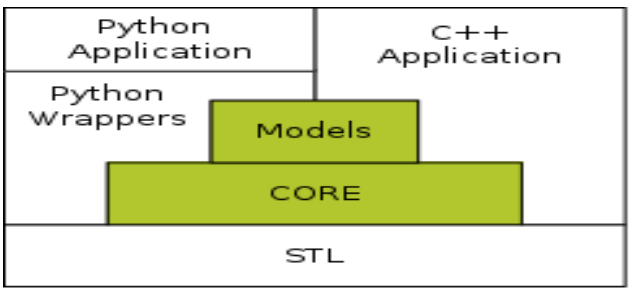
\includegraphics[width=5in]{figures/literature/ns3-architecture}
	\label{fig:ns3-architecture}
\end{figure}

\subsection{Robotics Simulator and Robotic Software}

Applications for physical robots can be created using robotics simulator without depending on the real hardware. This saves time and cost in the development of the application. Certain robotics simulator can render 3D model of robots and its environment, and can emulate robotic models, sensors, and control in virtual environment. They use physics engine to make the simulation more realistic.

\shortciteA{Staranowicz2011} has conducted a survey presenting comparison between the popular commercial and open-source robotic software for simulation and interfacing with real robots.  \shortciteA{Ivaldi2014} has conducted an online survey where participants present their feedback about the tools and use of dynamic simulation in robotics.

The most used robotics simulator are:
\begin{itemize}
	\item \textit{Gazebo.} Gazebo can simulate multiple robots in outdoor environments. It supports multiple physics engine. It can integrate with ROS using a set of ROS packages named gazebo\_ros\_pkgs. Gazebo is open source and free to use.
	\item \textit{ODE.} Open Dynamics Engine is a open-source physics library for simulating rigid body dynamics. It is used in computer games and simulation tools. It is open source.
	\item \textit{Bullet.} Bullet is an open-source physics library and is used in 3D animation software and game engines. It is open source.
	\item \textit{V-Rep.} V-Rep is a robot simulator software developed by Coppelia Robotics. It is free for academic usage. Commercial license is not free. 
	\item \textit{Webots.} Webots is an open-source robot simulator developed by Cyberbotics. It was open sourced in 2018. Robots can be modeled, programmed and simulated with the provided development environment.
\end{itemize}  

In this study, I intend to use Gazebo as the robotics simulator because:

\begin{itemize}
	\item The UAV firmware PixHawk provides SITL simulation for Gazebo and is the recommended option. 
	\item Gazebo supports PixHawk provided quad-copter (Iris).
	\item Gazebo supports multiple quad-copters.
	\item External world can be built in Gazebo using real world height maps.
	\item Gazebo supports sensors such as GPS and cameras.
	\item Gazebo can be integrated with ROS.
	\item Gazebo server provides API to integrate with other software. In my use case, I update the FANET nodes in ns-3 using the position provided by the robotics simulator. 
\end{itemize}

\section{Robot Operating System}
\shortciteA{Quigley2009} presents an overview of Robot Operating System (ROS). ROS is a framework for robotics software. It provides set of tools and communication layer on top of a host operating system, which helps in developing software for robotics. Availability of plethora of open source ROS packages avoids reinventing the wheel while developing the application.

ROS provides peer-to-peer connection to different processes of the robotics system. Each process is called a node and handles a specific aspect of the robotic system. The peer-to-peer topology makes use of a master node which enables the running nodes to find each other at run-time. Nodes exchange information with each other using messages. A message is a predefined strictly typed data structure. Nodes can exchange messages using either topic or service.

Nodes can publish message on a topic. Another node which uses the data generated by it can subscribe to the topic to receive messages. Nodes and topics have many-to-many association with each other. A single node can publish and subscribe to many topics and a topic may be published and subscribed by many nodes at once.

For synchronous communication, a node may call a service registered by another node. A node sends a request message to call a service and the node providing the service will reply with a response message. Unlike topics, service of a particular name can only be advertised by one node.

Nodes, topics and services can be grouped into namespaces. Topics and services follow URI reference naming convention. For example a topic that publishes GPS information for UAV 1 in a multi-UAV system may be named as \textit{/uav0/global\_position/gps}.

ROS has transformation system called tf/tf2. Tf2 is the new iteration of the transformation library. The transformation system helps the user keep track of multiple coordinate frames over time by using a tree structure to maintain relationship between coordinate frames. It allows for easy transformation of data between any two coordinate frames.

ROS has a wide array of tools for creating, debugging, inspecting and visualizing the data exchanged between the different nodes which speeds up the development.


\section{Multi-Agent Coverage Path Planning}

Coverage path planning (CPP) is the process of finding a suitable path that passes through a set of way-points in order to completely explore the area or volume of interest. The CCP problem is closely related to the lawnmower problem described by \shortciteA{Arkin2000}, and is proven to be NP-hard even for simple polygonal regions. Lawnmower problem is definded as finding a path/tour $\pi$ such that every point of the region $R$ is covered by some placement of the agent along $\pi$.

\shortciteA{Galceran2013}, on their survey of CPP methods mentions other closely related problems:

\begin{itemize}
	\item \textit{Covering salesman problem.} A generalization of the traveling salesman problem.
	\item \textit{Art gallery problem.} The minimum number of guards needed to station in a polygon area such that each point is visible to atleast one guard.
	\item \textit{Watchman route problem.} The shortest route in a polygon area such that each point is visible from the route.
\end{itemize}

All the above mentions problems are proven in general cases, to be NP-hard. Therefore, the solution to CPP problems are approximations to the problem.

Multiple agents can be helpful for the CPP task in many ways. Multiple agents can decrease the time taken to cover the area of interest and can be more robust as the exploration task can still be carried out if case of an agent failure. Multi-agent CPP is the process of finding a set of suitable paths through a set of way-points where the union of the found paths completely explore the area or volume of interest. 

\shortciteA{Almadhoun2019} has carried out an extensive survey for multi‑robot coverage path planning for model reconstruction and mapping. They classified the topics involved into:
\begin{itemize}
	\item Viewpoint generation,
	\item Coverage path planning approaches,
	\item Communication and task allocation, and
	\item Mapping.
\end{itemize}

Viewpoint generation can be generalized to generating potential way-points that can be used in coverage planning. Visiting all the  potential way-points will result in complete coverage of the area under scrutiny.

In another survey by \shortciteA{Xu2019}, which focuses on multi-agent coverage search, the topics have been classified as:
\begin{itemize}
	\item Environment modeling,
	\item Agent deployment, and
	\item Search Path Planning.
\end{itemize}

Environment modeling is a special case of viewpoint generation when the obstacles in the area to search is known beforehand. For unknown and dynamic environments, non-model based viewpoint generation is applied.

\subsection{Viewpoint Generation}

Viewpoint generation is the process of finding points or sub-regions in the area of interest. If all the viewpoints are visited by the participating agents, then complete coverage of the area is obtained. There are two methods in which viewpoints are generated, model based, and non-model based.

In model based viewpoint generation, prior information about the environment to survey is known.

In non-model based viewpoint generation, the next viewpoint is generated on the fly using real-time information about the environment.


\subsection{Coverage Path Planning Approaches}











\section{Structure from Motion}


\section{Chapter Summary}
All chapters except Chapter 1 must include an introductory paragraph/s and a chapter summary.

\FloatBarrier

